\documentclass[pdftex,12pt,a4paper]{report}

\usepackage[pdftex]{graphicx}
\usepackage{float}
\usepackage{fancyvrb}
\fvset{xleftmargin=2em}
\usepackage{graphicx}

\usepackage{pgfplots}
\pgfplotsset{width=10cm,compat=1.9}
\usepackage{tikzscale}
\usepackage{pgfplotstable}
\usepackage{booktabs}
\usepackage[font=small,labelfont=bf,tableposition=top]{caption}

\usepackage[utf8]{inputenc} % isto é um comentário
\usepackage[portuges]{babel}
%\usepackage[T1]{fontenc}
\usepackage{times}
%\usepackage{lmodern}
\usepackage[obeyspaces,spaces]{url}
\usepackage[left=25mm,right=25mm,top=25mm,bottom=25mm]{geometry}
\usepackage{titlesec}
\usepackage{mathtools}
%identa 1º paragrafo de capitulos e secções
\usepackage{indentfirst}
\usepackage{graphicx,color}
\newcommand{\HRule}{\rule{\linewidth}{0.5mm}}
\titleformat{\chapter}{\normalfont\huge}{\thechapter.}{20pt}{\huge}


\definecolor{verde}{rgb}{0,1,0}
\definecolor{azul}{rgb}{0,0,1}

\begin{document}

\begin{titlepage}


\begin{minipage}{0.3\textwidth}
\begin{flushleft} 

\includegraphics[width=\textwidth]{logo.png}
\end{flushleft}
\end{minipage}
\begin{minipage}{0.6\textwidth}
\begin{flushright} 

\textsc{Departamento de Engenharia Informática}\\[0.1cm]
\bfseries Mestrado Integrado em Engenharia Informática \\ [0.1cm]
\bfseries \textit{Laboratórios de Informática III}\\[8mm]

\end{flushright}
\end{minipage}


\vspace{3cm}


\begin{center}


\LARGE Gestão de Vendas de uma cadeia de Distribuição com 3 filiais

\Large \textbf{GEREVENDAS}\\[1.5cm]


{\Large \bfseries Grupo 84\\[2cm] }


\noindent\begin{minipage}[b]{.1\textwidth}
	
\includegraphics[scale=0.12123]{celia}
	\small{Célia Figueiredo a67637}
\end{minipage} 
\hfill
\begin{minipage}[b]{.1\textwidth}
	
\includegraphics[scale=0.1]{gil}
	\small{Gil Gonçalves a67738}
\end{minipage}
\hfill
\begin{minipage}[b]{.1\textwidth}
	
\includegraphics[scale=0.1]{humberto}
	\small{Humberto Vaz a73236 }
\end{minipage} 
\hfill
\begin{minipage}[b]{.1\textwidth}	
\includegraphics[scale=0.1]{ricardo}
		\small{Ricardo Lopes a72062}
\end{minipage}



\vspace{3ex}


\vfill

\large Braga, {\large \today}

\end{center}
\end{titlepage}

\chapter{Introdução}

No âmbito da unidade curricular de Laboratórios de Informática III do 2ºano da licenciatura de Engenharia Informática foi proposto o desenvolvimento de um projeto em linguagem C que tem por objetivo fundamental ajudar à consolidação dos conteúdos teóricos e práticos e enriquecer os conhecimentos adquiridos nas UCs de Programação Imperativa, de Algoritmos e Complexidade, e da disciplina de Arquitetura de Computadores.Este projeto considera-se um grande desafio para nós pelo facto de passarmos a realizar programação em grande escala, uma vez que se trata de grandes volumes de dados e por isso uma maior complexidade. Nesse sentido, o desenvolvimento deste programa será realizado à luz dos princípios da modularidade (divisão do código fonte em unidades separadas coerentes) e do encapsulamento (garantia de proteção e acessos controlados aos dados). 


\tableofcontents

\chapter{Descrição dos Módulos}

A arquitetura da aplicação a desenvolver é definida por quatro módulos principais: Catálogo de clientes, Catálogo de produtos, Faturação Global e Vendas por Filial, cujas fontes de dados são três ficheiros de texto detalhados abaixo.
 
\paragraph{}
No ficheiro \textbf{Produtos.txt} cada linha representa o código de um produto vendável no hipermercado, sendo cada código formado por duas letras maiúsculas e 4 dígitos (que representam um inteiro entre 1000 e 1999), como no exemplo: 

\begin{verbatim}
AB9012
XY1185
BC9190
\end{verbatim}

O ficheiro de produtos contém cerca de 200.000 códigos de produto. 

\paragraph{}
No ficheiro \textbf{Clientes.txt} cada linha representa o código de um cliente identificado no hipermercado, sendo cada código de cliente formado por uma letra maiúscula e 4 dígitos que representam um inteiro entre 1000 e 5000, segue um exemplo: 

\begin{Verbatim}
F2916
W1219
F2915
\end{Verbatim}

O ficheiro de clientes contém cerca de 20.000 códigos de cliente. 

\paragraph{}
O ficheiro \textbf{Vendas\_1M.txt}, no qual cada linha representa o registo de uma venda efectuada numa qualquer das 3 filiais da Cadeia de Distribuição. Cada linha (a que chamaremos compra ou venda, o que apenas depende do ponto de vista) será formada por um código de produto, um preço unitário decimal (entre 0.0 e 999.99), o número inteiro de unidades compradas (entre 1 e 200), a letra \textbf{N} ou \textbf{P} conforme tenha sido uma compra \textbf{Normal} ou uma compra em \textbf{Promoção}, o código do cliente, o mês da compra (1 .. 12) e a filial (de 1 a 3) onde a venda foi realizada, como se pode verificar nos exemplos seguintes:
 
 \begin{Verbatim}
KR1583 77.72 128 P L4891 2 1
QQ1041 536.53 194 P X4054 12 3
OP1244 481.43 67 P Q3869 9 1
JP1982 343.2 168 N T1805 10 2
IZ1636 923.72 193 P T2220 4 2 
 \end{Verbatim}
 
 
O ficheiro de vendas inicial, \textbf{Vendas\_1M.txt} , conterá 1.000.000 (1 milhão) de registos de vendas realizadas nas 3 filiais da cadeia de distribuição. Existirão também os ficheiros  \textbf{Vendas\_3M.txt} e  \textbf{Vendas\_5M.txt} utilizados para as questões de performance da aplicação. 

\newpage 
\paragraph{}
A aplicação possuiu uma arquitectura tal como apresentado na figura seguinte, em que se identificam as fontes de dados, a sua leitura e os módulos de dados a construir: 



\begin{figure}[h!]
	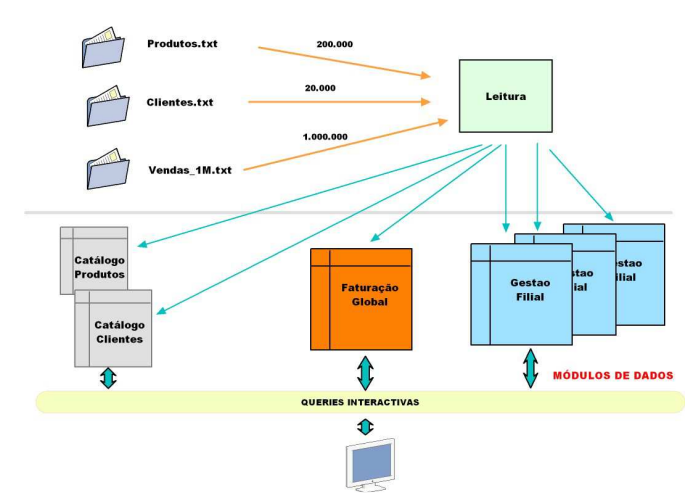
\includegraphics[scale=0.8]{arquiteturaproj.png}  
	\caption{Arquitetura da aplicação}  
\end{figure}



\section{Catálogo de Clientes}
É o módulo de dados onde são guardados os códigos de todos os clientes do ficheiro \textbf{Clientes.txt}, organizados por índice alfabético; 

\subsection{Clientes.h}

Módulo de dados onde são guardados os códigos de todos os clientes do ficheiro \textbf{Clientes.txt}. O array de árvores este que é um array de 26 posições cujos índices se encontram organizados alfabeticamente. Cada índice contém um apontador para uma árvore correspondente à letra respetiva desse índice.

\subsubsection{Tipos Opacos}

\begin{Verbatim}
typedef struct catalogo_clientes *CatClientes;
\end{Verbatim}

\textbf{clientes.c}
\begin{verbatim}
struct catalogo_clientes{
ARVORE indices[27];
};
\end{verbatim}

O typedef no ficheiro Clientes.h é a única informação que o utilizador têm relativamente à implementação de dados, não tendo acesso ao ficheiro .c dos clientes, não conseguindo conhecer a verdadeira implementação da estrutura avl.Deste modo garantimos o encapsulamento de dados e a única forma de o utilizador interagir com o catálogo de clientes será através da API; 

\subsubsection{/*API*/}

\begin{itemize}

\item CatClientes inicializa\_catalogo\_clientes() - Função que cria uma estrutura de clientes vazia;

\item void insertC(CatClientes c, char * valor) - insere um dado cliente na estrutura CatClientes, de maneira ordenada alfabeticamente; 

\item void cat\_remove\_cliente(CatClientes cat, char *str) - remove um cliente da estrutura CatCliente 

\item void free\_catalogo\_Clientes(CatClientes cat) - função que liberta todo o espaço ocupado pela estrutura CatClientes

\item int existeCliente (char *cliente,CatClientes cat) - função que verifica se um cliente existe
\item int numeroClientes(CatClientes cat) - função que conta todos os nodos

\item int numeroClientesLetra(CatClientes cat, char letra) - função que conta os nodos por que começam por determinada letra


\end{itemize}

\section{Catálogo de Produtos}

 Módulo de dados onde são guardados os códigos de todos os produtos do ficheiro \textbf{Produtos.txt}, organizados por índice alfabético, o que irá permitir, de forma eficaz, saber quais são os produtos cujos códigos começam por uma dada letra do alfabeto, quantos são



\subsection{Produtos.h}

\subsubsection{Tipos Opacos}
\begin{verbatim}
typedef struct catalogo_produtos *CatProdutos;
\end{verbatim}

\textbf{produtos.c}

\begin{verbatim}
struct catalogo_produtos{
ARVORE indices[27];
};
\end{verbatim}

\subsubsection{/*API*/}

\begin{itemize}
	
\item CatProdutos inicializa\_catalogo\_produtos();
\item void insertP(CatProdutos c, char * valor);
\item void cat\_remove\_produto(CatProdutos cat, char *str);
\item void free\_catalogo\_produtos(CatProdutos cat);
\item int existeProduto (char *produto,CatProdutos cat);
\item int numeroProdutos(CatProdutos cat);
\item int numeroProdutosLetra(CatProdutos cat, char letra);
\item ARRAY listaProdutosLetra(CatProdutos cat, char l);
\end{itemize}


\section{Faturação Global}

Módulo de dados que contém as estruturas de dados responsáveis pela resposta eficiente a questões quantitativas que relacionam os produtos às suas vendas mensais, em modo Normal (N) ou em Promoção (P), para cada um dos casos guardando o número de vendas e o valor total de faturação de cada um destes tipos. Este módulo refecencia todos os produtos, mesmo os que nunca foram vendidos, não contém qualquer referência a clientes, mas é capaz de distinguir os valores obtidos em cada filial; 

\subsection{faturacao.h}

\subsubsection{Tipos Opacos}
\begin{Verbatim}
typedef struct faturacao *Faturacao;
typedef struct info *Info;
\end{Verbatim}

\textbf{faturacao.c}
\begin{verbatim}
struct faturacao{
int totalvendas[12];
float totalfaturado[12];
ARVORE produtos;
};

struct info{
char *code;
int vendasP[12][3];
int vendasN[12][3];
float faturadoN[12][3];
float faturadoP[12][3];
int quantidadeP[12][3];
int quantidadeN[12][3];
};
\end{verbatim}

\subsubsection{/*API*/}

\begin{itemize}

\item	Faturacao inicializa\_faturacao();
\item	void cont\_regista\_produto(Faturacao fat, char *prod);
\item	void cont\_insere\_venda(Faturacao fat, char *produto, int q, float preco, char M,int mes, int filial);
\item	void cont\_remove\_produto(Faturacao fat, char *produto);
\item	void free\_faturacao(Faturacao fat);
\item	int getNumeroTotalVendasNTodasFiliais (char* prod,int mes,Faturacao fat);
\item	int getNumeroTotalVendasNFilialX (char* prod,int mes,Faturacao fat, int filial);
\item	int getNumeroTotalVendasPTodasFiliais (char* prod,int mes,Faturacao fat);
\item	int getNumeroTotalVendasPFilialX (char* prod,int mes,Faturacao fat, int filial);
\item	float getTotalFatPFilialX (char* prod,int mes,Faturacao fat, int filial);
\item	float getTotalFatNFilialX (char* prod,int mes,Faturacao fat, int filial);
\item	int getVendasNFilialX (char* prod,int mes,Faturacao fat, int filial);
\item	int getVendasPFilialX (char* prod,int mes,Faturacao fat, int filial);
\item	int getQuantidadeNFilialX (char* prod,int mes,Faturacao fat, int filial);
\item	int getQuantidadePFilialX (char* prod,int mes,Faturacao fat, int filial);
\item	ARRAY naoCompradosFilial(Faturacao fat, int filial);
\item	ARRAY naoComprados(Faturacao fat);
\item	int totalVendasMeses(Faturacao fat, int a, int b);
\item	float totalFatMeses(Faturacao fat, int a, int b);
\item	ARRAY nMaisVendidos(Faturacao fat, int n);
\item	int getQuantidadeFilial(Faturacao fat, char*prod, int filial);
	
\end{itemize}


\section{Gestão da Filial}


Módulo de dados que, a partir dos ficheiros lidos, contém as estruturas de dados adequadas à representação dos relacionamentos, fundamentais para a aplicação, entre produtos e clientes, ou seja, para cada produto, saber quais os clientes que o compraram, quantas unidades cada um comprou, em que mês e em que filial.

 Para a estruturação optimizada dos dados deste módulo de dados tivemos em atenção que pretendemos ter o histórico de vendas organizado por filiais para uma melhor análise, nunca esquecendo que existem 3 filiais nesta cadeia. 

\subsection{Filial.h}

\subsubsection{Tipos Opacos}
\begin{Verbatim}
typedef struct filial *Filial;
typedef struct icliente *Icliente;
typedef struct iprodutos *Iprodutos;
\end{Verbatim}

\textbf{Filial.c}
\begin{verbatim}
struct filial{
ARVORE infoCliente;
};

struct icliente{
char *cliente;
int quantidade[12];
ARVORE infoprodutos[2];
};

struct iprodutos{
char *prod;
int quantidadeT;
float gastouT;
int quantidade[12];
float gastou[12];
};
\end{verbatim}

\subsubsection{}

\begin{itemize}
\item	Filial inicializa\_filial();
\item	void fil\_regista\_cliente(Filial fil, char *cliente);
\item	void fil\_insere\_prod(Filial fil, char *cliente, char *produto,int q, int mes, float preco, char p);
\item	int getQuantidadeMesCliente(Filial fil, char *cliente, int mes);
\item	ARRAY naoCompraram(Filial fil);
\item	ARRAY compraram(Filial fil);
\item	void clientesCompraram(Filial fil,ARRAY a);
\item	void free\_filial(Filial fil);
\item	ARRAY topMaisGastou(ARRAY a);
\item	ARRAY clientesCompraramProduto(Filial fil, char* produto);
\item	int comprouProdutoN(Filial fil, char* cliente, char* produto);
\item	int comprouProdutoP(Filial fil, char* cliente, char* produto);
\item	int getNumClientesFilial(Filial fil, char* produto);
\item	void getIProdMes(Filial fil, char* cliente, int mes, ARRAY a);
\item	ARRAY extraiPorQuantidade(ARRAY a,int mes);
\item	void removeNaoCompraram(Filial fil, ARRAY a);
\item	void removeCompraram(Filial fil, ARRAY a);
\end{itemize}


\chapter{Main.c}




\chapter{Interface do utilizador}
Quando o utilizador executa o programa é-lhe pedido que escolha qual o documento de texto que pretende analisar, como podemos observar na figura seguinte: 

\begin{figure}[h!]
	\centering
	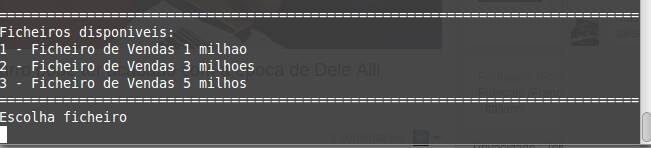
\includegraphics[scale=0.4]{1querie.png}  
	\caption{Escolha do ficheiro de vendas a analisar}  
\end{figure}

O ficheiro é carregado e de seguida aparece um menu com 12 opções, referentes às 12 queries do projeto, sendo que decidimos usar o [0] para sair do GereVendas. O objetivo é que o utilizador prima a tecla correspondente à opção do menu pretendida.

\begin{figure}[h!]
	\centering
	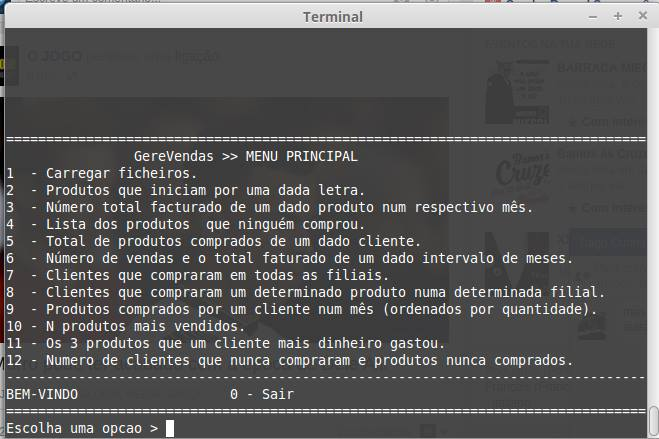
\includegraphics[scale=0.6]{menu.png}  
	\caption{Menu principal da aplicação}  
\end{figure}



\chapter{Resultados e comentários sobre os testes de performance}
Depois de desenvolver e codificar todo o projeto foi-nos proposto realizar alguns testes de performance que consistem em comparar os tempos de execução das queries 8, 9, 10, 11 e 12 usando os ficheiros Vendas\_1M.txt ( 1000 000 vendas), Vendas\_3M.txt (3 milhões de vendas) e Vendas\_5M.txt (5 milhões de vendas).
Uma vez que a quantidade de vendas vai aumentando de ficheiro para ficheiro é aceitável que os tempos de execução para os carregar aumente.


\begin{figure}[h!]
	\centering
	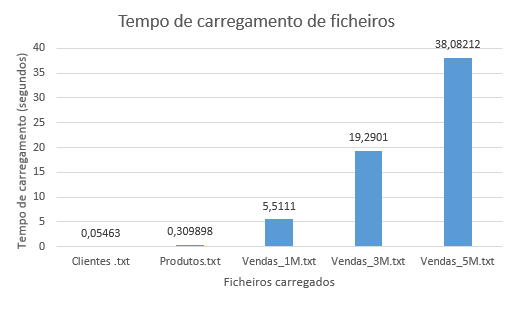
\includegraphics[scale=0.8]{grafcarregamento.png}  
	\caption{Gráfico do tempo de execução do carregamento dos 3 ficheiros de vendas}  
\end{figure}

Comparando os valores de execução das queries pretendidas, como podemos observar nos respetivos gráficos apresentados,




\chapter{Makefile e Grafo de dependências}
A makefile permite correr todo o software escrevendo apenas \textit{“make”} no terminal. Posto isto, apresenta-se a makefile utilizada cujas flags utilizadas como opção de compilação são –Wall –Wextra –ansi – pedantic –O2.
Possui ainda a opção “make clean” que elimina todos os “.o” que foram criados quando se compilou o software.

\begin{figure}[h!]
	\centering
	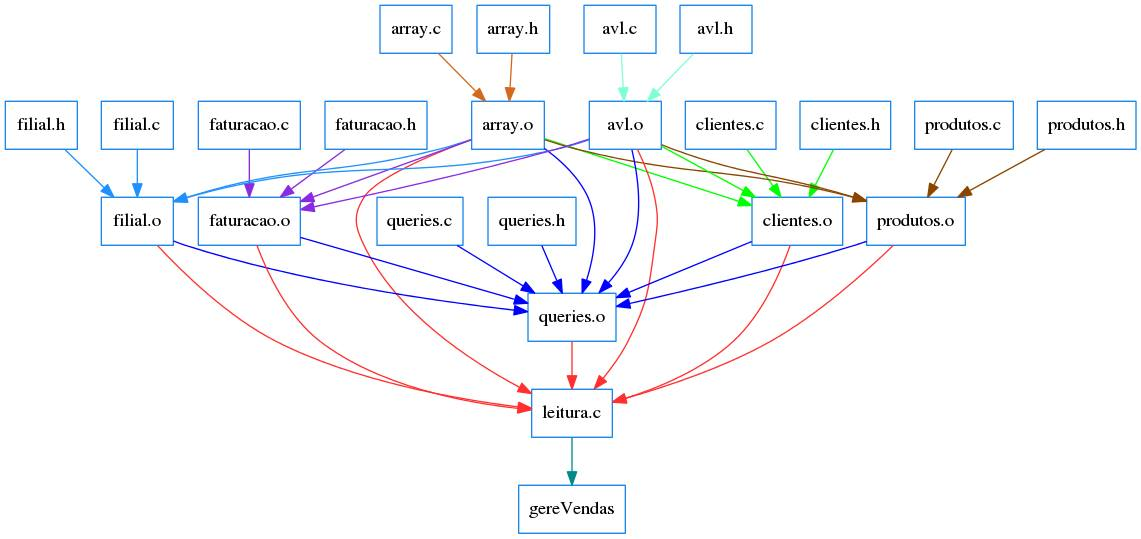
\includegraphics[scale=0.4]{grafodependencias.png}  
	\caption{Grafo de depêndencias}  
\end{figure}

\begin{verbatim}
objects = array.o avl.o clientes.o faturacao.o filial.o \
produtos.o queries.o 

CFLAGS=-Wall -ansi -pedantic -O2

all:
make clean
make produtos
make array
make avl
make clientes
make faturacao
make filial
make queries
make leitura

leitura: src/leitura.c array.o avl.o clientes.o faturacao.o filial.o
 produtos.o queries.o 
gcc src/leitura.c array.o avl.o clientes.o faturacao.o filial.o
 produtos.o queries.o $(CFLAGS) -o gereVendas -lm

queries: src/queries.c src/headers/queries.h
gcc src/queries.c -c $(CFLAGS)

clientes: src/clientes.c src/headers/clientes.h
gcc src/clientes.c -c $(CFLAGS)

produtos: src/produtos.c src/headers/produtos.h
gcc src/produtos.c -c $(CFLAGS)

array: src/array.c src/headers/array.h
gcc src/array.c -c $(CFLAGS)

faturacao: src/faturacao.c src/headers/faturacao.h
gcc src/faturacao.c -c $(CFLAGS)

filial: src/filial.c src/headers/filial.h
gcc src/filial.c -c $(CFLAGS)

avl: src/avl.c src/headers/avl.h
gcc src/avl.c -c $(CFLAGS)

.PHONY : clean
clean :
rm -f gereVendas
rm -f $(objects)
rm -f gesval
\end{verbatim}


\chapter{Conclusão}

Uma vez que se tratou de um trabalho de uma dimensão já considerável comparando com o que estávamos habituados envolveu utilização de técnicas particulares e tivemos sempre como objetivo que este trabalho fosse concebido de modo a que seja facilmente modificável, e seja, apesar da complexidade, o mais optimizado possível a todos os níveis.

Inicialmente, tivemos dificuldades nas AVLs pois estávamos a fazer uma AVL para cada módulo. Depois de alguns problemas com o seu balanceamento, acabamos por apostar na utilização da biblioteca standard AVL da GNU, que nos facilitou não só o carregamento dos ficheiros em memória, mas também na realização de algumas queries, devido ao vasto conjunto de úteis funções que a biblioteca contém, evitando assim a repetição de código. 



\end {document}


